\documentclass[11pt]{article}
% Remove the "review" option (or change to "[review]") to switch versions.
% No option = final / camera-ready (no line numbers, no page numbers).
\usepackage[final]{acl}
% Standard package includes
\usepackage{times}
\usepackage{latexsym}
\usepackage[T1]{fontenc}
\usepackage[utf8]{inputenc}
\usepackage{microtype}
\usepackage{inconsolata}
\usepackage{graphicx}
% --- Black & white schematics (use the document font) ---
\usepackage{tikz}
\usetikzlibrary{arrows.meta,positioning,fit,calc}
% Monochrome TikZ styles: white / light-grey fills, black strokes only.
\tikzset{
  box/.style   = {draw=black, rounded corners=1.5pt, align=center,
                  inner sep=3pt, font=\footnotesize, fill=white},
  boxg/.style  = {draw=black, rounded corners=1.5pt, align=center,
                  inner sep=3pt, font=\footnotesize, fill=black!8},
  lab/.style   = {font=\scriptsize\itshape, align=center},
  arr/.style   = {-{Latex[length=2mm]}, draw=black, thick},
  darr/.style  = {-{Latex[length=2mm]}, draw=black, thick, dashed},
}
\title{HERA: A Conversational Copilot for Identifying Ethical and\\
       Regulatory Risks in Health Apps}
\author{Nathan Massicot \\
        MSE Data Science, Bern University of Applied Sciences \\
        Quellgasse 21, 2502 Biel, Switzerland \\
        \texttt{nathan2massicot@gmail.com} \\
        \\
        \small Specialisation Project~2, Supervisor: Prof.\ Dr.\ Kerstin Denecke}
\begin{document}
\maketitle
\begin{abstract}
The moment a piece of software touches health, it enters a maze of rules: data
protection, medical-device law, artificial-intelligence regulation, accessibility.
These frameworks overlap, change quickly, and differ from one country to the next,
so ethical and regulatory risks are often noticed too late. After launch, when they
are costly to fix and sometimes dangerous for patients. In this context, we present HERA Copilot
(Health Ethical \& Regulatory Assessment), a conversational copilot that helps a
mobile-health (mHealth) app developer spot these risks early, right from the design
stage. HERA rests on a new taxonomy that merges eight regulatory and ethical
frameworks into seven pillars and thirty-eight dimensions. We transformed official
regulatory texts into short structured ``cards'', linked every taxonomy dimension to
the rules that apply to it, and generated training dialogues from this knowledge base.
On top of one small, locally-run language model we implemented and compared four
architectures: a prompt-only baseline, a fine-tuned model (QLoRA), retrieval-augmented
generation (RAG), and a multi-agent setup. All four were evaluated on twenty-five
realistic app scenarios with a reproducible ``simulated developer'', automatic
coverage metrics, and an LLM judge. RAG gave the most useful and best-grounded advice;
the prompt-only baseline was a fast and solid fallback; the multi-agent setup was
slower with no clear gain; and the fine-tuned model collapsed, a result we trace to
data and hardware limits rather than to the method itself.
\end{abstract}
\section{Introduction}
The moment an app is related health, it enters a maze of frameworks. A single mobile
health application can fall at once under data-protection law, the rules for medical
devices, the new regulation on artificial intelligence, and accessibility standards.
In Europe these include the General Data Protection Regulation \citep{gdpr2016}, the
Medical Device Regulation \citep{mdr2017}, the Artificial Intelligence Act
\citep{euaiact2024}, and quality standards for health apps such as ISO/TS~82304-2
\citep{iso82304}. These texts overlap, they are revised often, and they differ from one
country to the next: a health app sold in the European Union, in Switzerland and in the
United Kingdom faces three partly different rule sets.
Developers are neither lawyers nor ethicists, so it is difficult for them to know what actually applies to their
product. The frameworks that could help already exist, but they are scattered and
written for experts; none of them is designed to guide a developer, step by step,
through the questions they should be asking. As a consequence, risks tend to surface
late. After the product is live when fixing them is expensive and, in a health
setting, potentially dangerous. What is missing is not another regulation but a tool
that helps a developer think about these issues upfront, in a structured and
reasonably complete way.
Our answer is a copilot that asks the right questions from the design stage. The system
is built around HERA (Health Ethical \& Regulatory Assessment), a taxonomy that
unifies eight regulatory and ethical frameworks into a single, actionable structure that
applies to health apps with or without AI. A conversational assistant uses this taxonomy
to interview the developer one question at a time, dig into the specifics of their app,
name concrete risks together with the precise regulation that applies, and finally
produce a structured risk report. The idea of organising risk reasoning around an
explicit, structured taxonomy and a small team of cooperating language-model
``agents'' is adapted from \citet{deng2025ethical}, who applied it to ethical awareness
in finance; we re-target it at digital health.
This report makes four contributions. (i) We describe how we collected official
regulatory texts and turned them into a small, structured knowledge base of regulatory
cards (Section~\ref{sec:hera}). (ii) We present the HERA taxonomy : seven
pillars, thirty-eight dimensions and the per-dimension ``fiches'' that link each
dimension to the rules that govern it. (iii) We implement four copilot
architectures on top of the same small, locally-run model and explain how each
one was chosen, with its strengths and weaknesses (Section~\ref{sec:arch}).
(iv) We define a reproducible evaluation that compares the four approaches on
twenty-five realistic scenarios using a simulated developer, automatic metrics, and an
LLM judge (Section~\ref{sec:eval}), and we report and discuss the results
(Sections~\ref{sec:results}--\ref{sec:discussion}). Our headline finding is that
retrieval-augmented generation gives the most useful advice, and that the disappointing
fine-tuned model failed because of our training method limited by hardware.
\section{Building HERA: from regulations to a structured knowledge base}
\label{sec:hera}
Before any model can give advice, it needs the right knowledge in the right shape. This
section describes how we gathered the regulatory material, how we organised it into the
HERA taxonomy, how we linked each part of the taxonomy to the rules that apply, and how
we produced the training dialogues. Figure~\ref{fig:pipeline} summarises the pipeline.
\begin{figure}[t]
\centering
\resizebox{0.92\columnwidth}{!}{%
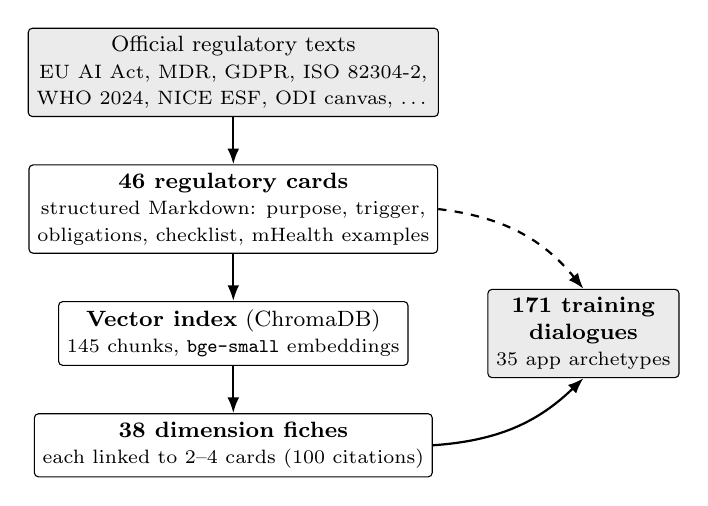
\begin{tikzpicture}[node distance=6mm and 0mm]
  \node[boxg] (src) {Official regulatory texts\\\scriptsize EU AI Act, MDR, GDPR, ISO~82304-2,\\\scriptsize WHO~2024, NICE ESF, ODI canvas, \ldots};
  \node[box, below=of src] (cards) {\textbf{46 regulatory cards}\\\scriptsize structured Markdown: purpose, trigger,\\\scriptsize obligations, checklist, mHealth examples};
  \node[box, below=of cards] (index) {\textbf{Vector index} (ChromaDB)\\\scriptsize 145 chunks, \texttt{bge-small} embeddings};
  \node[box, below=of index] (fiches) {\textbf{38 dimension fiches}\\\scriptsize each linked to 2--4 cards (100 citations)};
  \node[boxg, right=10mm of index] (dlg) {\textbf{171 training}\\\textbf{dialogues}\\\scriptsize 35 app archetypes};
  \draw[arr] (src) -- (cards);
  \draw[arr] (cards) -- (index);
  \draw[arr] (index) -- (fiches);
  \draw[arr] (fiches.east) to[bend right=20] (dlg.south);
  \draw[darr] (cards.east) to[bend left=22] (dlg.north);
\end{tikzpicture}}
\caption{Knowledge-base construction. Official texts are summarised into regulatory
cards, indexed in a local vector database, and linked to the taxonomy dimensions; the
same material seeds the synthetic training dialogues.}
\label{fig:pipeline}
\end{figure}
\subsection{From scattered regulations to regulatory cards}
We started from the frameworks that practitioners already rely on. The selection was
guided by the DTX Risk Assessment Canvas \citep{denecke2023dtx}, the World Health
Organization guidance on AI for health \citep{who2024aihealth}, the four principles of
biomedical ethics \citep{beauchamp2019principles}, and the main European legal texts
\citep{euaiact2024,mdr2017,gdpr2016,iso82304}, complemented by the NICE evidence
standards for digital health \citep{nice2022esf}. In total we catalogued
fourteen primary documents in a single manifest that records, for each entry,
its title, publisher, jurisdiction, key articles, official URL, licence, and an access
record (SHA-256 hash and retrieval date). The manifest is the single source of truth for
provenance: it makes every downstream claim traceable back to a dated, identifiable
source.
Reading fourteen long legal documents is exactly the burden a developer cannot carry, so
we compressed the relevant content into 46 short regulatory cards. Each card
is a plain-text (Markdown) file with a fixed structure: what the rule is about, when it
is triggered, the concrete obligations it imposes, a short checklist, a few examples
specific to mHealth, and pointers to related cards. A card on the Medical Device
Regulation, for instance, explains in a few lines when an app counts as a medical device,
which class it is likely to be, and what that means in practice. The cards are the
human-readable backbone of the whole system: they are easy to read, easy to keep up to
date, and easy for a model to retrieve and cite.
Provenance also dictated what we were allowed to store. Most of the corpus is openly
licensed EU Official Journal regulations and Swiss federal law (Fedlex) are in the
public domain, MDCG guidance is free to use with attribution, WHO documents are released
under CC~BY-NC-SA, and NICE/NHS material is free for non-commercial use so the primary
texts could be retained and indexed directly. Paywalled standards are the exception.
ISO/IEC~82304-2, for instance, is not freely distributable, and we therefore adopted a
deliberate cite, do not store policy: no copyrighted standard is downloaded,
ingested, or redistributed. This is workable because a standard can be cited
authoritatively from its public metadata alone (its number, title, scope, section
structure, and catalogue URL ) while its substantive content is reconstructed from freely
available secondary sources that paraphrase it. The copilot thus
knows ISO~82304-2 through what open documents say about it, never through the
protected text itself; in the manifest such entries carry an empty file field and an
explicit licence note, and no standard PDF is ever committed to the repository.
\subsection{The HERA taxonomy: seven pillars, thirty-eight dimensions}
The cards tell a developer about individual rules, but they do not by themselves provide
a map of everything that should be checked. That map is the HERA taxonomy, and it
grew directly out of a gap we met while writing the cards: each source framework
illuminated only one facet of the problem,the DTX canvas framed risk, the WHO guidance
addressed AI ethics, Beauchamp and Childress supplied the bioethical principles, the
European legal texts defined compliance, and NICE set the evidence bar, yet none offered
a single, operational checklist a developer could work through. We therefore synthesised
one. By reading across the frameworks and grouping recurring concerns, we organised the
field into seven pillars : patient safety, data \& privacy, patient autonomy,
quality \& usability, transparency, equity, and regulatory governance and then
decomposed each pillar into concrete, checkable dimensions, for a total of
thirty-eight (Table~\ref{tab:taxonomy}). Crucially, every pillar applies to non-AI apps
as well: a simple medication reminder still raises autonomy, privacy and reliability
concerns without any algorithm.
Each dimension is written up as a small ``fiche'' (Figure~\ref{fig:taxo}) with a fixed
shape: a short identifier such as \texttt{[P2.D3]}, a name, a one-sentence plain-language
description, a handful of reflection questions, the risks that typically arise, and
concrete mitigation ideas. This fixed shape is what lets the copilot move smoothly from a
question (``where is the data stored?'') to a named risk (``\texttt{[P2.D3]} unencrypted
health data'') to a usable mitigation (``encrypt at rest and document the lawful basis
under GDPR Art.~9'').
\begin{figure}[t]
\centering
\resizebox{0.96\columnwidth}{!}{%
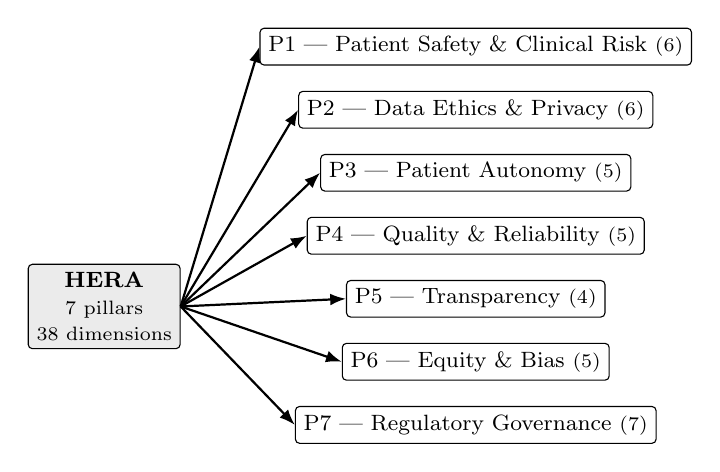
\begin{tikzpicture}[node distance=3.2mm]
  \node[boxg] (root) {\textbf{HERA}\\\scriptsize 7 pillars\\\scriptsize 38 dimensions};
  \node[box, right=10mm of root, yshift=33mm] (p1) {P1 --- Patient Safety \& Clinical Risk \scriptsize(6)};
  \node[box, below=of p1] (p2) {P2 --- Data Ethics \& Privacy \scriptsize(6)};
  \node[box, below=of p2] (p3) {P3 --- Patient Autonomy \scriptsize(5)};
  \node[box, below=of p3] (p4) {P4 --- Quality \& Reliability \scriptsize(5)};
  \node[box, below=of p4] (p5) {P5 --- Transparency \scriptsize(4)};
  \node[box, below=of p5] (p6) {P6 --- Equity \& Bias \scriptsize(5)};
  \node[box, below=of p6] (p7) {P7 --- Regulatory Governance \scriptsize(7)};
  \foreach \p in {p1,p2,p3,p4,p5,p6,p7}{\draw[arr] (root.east) -- (\p.west);}
\end{tikzpicture}}
\vspace{4pt}
\resizebox{0.96\columnwidth}{!}{%
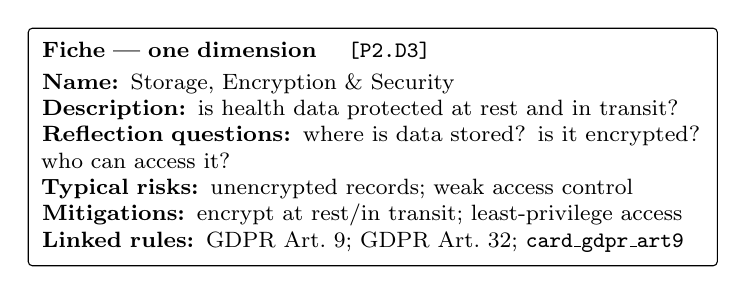
\begin{tikzpicture}
  \node[box, align=left, text width=8.4cm, inner sep=5pt] (f) {%
    \textbf{Fiche --- one dimension} \quad \texttt{[P2.D3]}\\[2pt]
    \textbf{Name:} Storage, Encryption \& Security\\
    \textbf{Description:} is health data protected at rest and in transit?\\
    \textbf{Reflection questions:} where is data stored? is it encrypted? who can access it?\\
    \textbf{Typical risks:} unencrypted records; weak access control\\
    \textbf{Mitigations:} encrypt at rest/in transit; least-privilege access\\
    \textbf{Linked rules:} GDPR Art.~9; GDPR Art.~32; \texttt{card\_gdpr\_art9}%
  };
\end{tikzpicture}}
\caption{Top: the HERA taxonomy --- one root, seven pillars, thirty-eight dimensions
(dimension count in parentheses). Bottom: the structure of a single dimension fiche,
which links a taxonomy entry to the regulatory cards that apply to it.}
\label{fig:taxo}
\end{figure}
\begin{table*}[t]
  \centering
  \footnotesize
  \setlength{\tabcolsep}{4pt}
  \begin{tabular}{|p{3.0cm}|p{12.3cm}|}
    \hline
    \textbf{Pillar} & \textbf{Dimensions} \\
    \hline
    P1 --- Patient Safety \& Clinical Risk &
    Clinical Evidence \& Validation; Contraindications \& Adverse Effects; False Sense of
    Security; Delayed Medical Consultation; Measurement Reliability; System Dependency \&
    Over-reliance \\
    \hline
    P2 --- Data Ethics \& Privacy &
    Informed Consent; Data Minimization; Storage, Encryption \& Security; Third-Party Data
    Sharing; Anonymization \& Right to Erasure; Vulnerable Population Data \\
    \hline
    P3 --- Patient Autonomy \& Therapeutic Relationship &
    Right to Make Decisions; Emotional Manipulation \& Excessive Nudging; Impact on
    Doctor--Patient Relationship; Dynamic Consent \& Withdrawal Rights; Automation Bias \\
    \hline
    P4 --- Quality, Usability \& Technical Reliability &
    App Stability \& Error Handling; Interoperability \& Data Exchange; Accessibility
    (WCAG, literacy, language); User-Centered Design \& Usability Testing; Offline
    Functionality \& Updates \\
    \hline
    P5 --- Transparency \& Explainability &
    Understandable Output; Clear Communication of Limitations; Decision Traceability \&
    Logging; Distinction Clinically-validated vs Estimated Content \\
    \hline
    P6 --- Equity, Bias \& Social Justice &
    Data \& Clinical Rule Bias; Digital Divide \& Socioeconomic Access; Cross-Cultural \&
    Multilingual Validation; Impact on Existing Health Inequalities; Representativeness in
    Validation Studies \\
    \hline
    P7 --- Regulatory Compliance \& Governance &
    Medical Device Classification (SaMD); CE Marking \& MDR Conformity; EU AI Act Risk
    Classification; GDPR Compliance (DPO/DPIA); Post-Market Surveillance \& Vigilance;
    Third-Party Audit \& Certification; Lifecycle \& Documentation Management \\
    \hline
  \end{tabular}
  \caption{The HERA taxonomy: seven pillars and their thirty-eight dimensions.}
  \label{tab:taxonomy}
\end{table*}
\subsection{Linking dimensions to the rules that apply}
We still needed a reliable bridge between an abstract dimension (``Storage, Encryption \&
Security'') and the specific cards that govern it. Doing this by hand for thirty-eight
dimensions would be slow and subjective, so we used retrieval. We indexed the 46
cards in a local vector database (ChromaDB), splitting each card into short overlapping
passages and turning every passage into a numerical vector with a sentence-embedding
model \citep{reimers2019sentencebert,xiao2024cpack}. For each dimension we then searched
the index using the dimension's name and reflection questions, and kept the closest
cards. A short curation pass kept only the two to four cards that were genuinely
relevant, each with a one-line explanation of why it applies. The result is a set
of thirty-eight ``source fiches'' (one for each dimension) carrying one hundred citations in total becoming the
machine-readable link between the taxonomy and the regulatory text.
\subsection{Synthetic training dialogues}
Finally, to be able to train a small model to use correctly HERA, we needed
examples of the target behaviour. We wrote thirty-five app ``archetypes'' idea (a diabetes
tracker, a mental-health chatbot, an AI symptom checker, and so on, each tagged with its
category, data sensitivity and target markets) and used them to generate
171 multi-turn dialogues. Twenty-one of these were written by hand; they then served as a 21-shot set
of exemplars from which a state-of-the-art LLM generated the remaining 150. In every dialogue a developer describes an app and the
copilot asks reflection questions one at a time, citing dimension identifiers such as
\texttt{[P1.D2]}, and closes with a short structured risk report. Each dialogue was
checked against a strict format schema and de-duplicated. This set is the training
material for the fine-tuned approach and the behavioural template that all four
architectures imitate.
\section{Copilot architectures}
\label{sec:arch}
With the knowledge base in place, the central question of the project was: what is
the best way to turn this knowledge into good conversational advice? We implemented four
architectures and compared them head to head. Figure~\ref{fig:arch} shows the four side
by side.
\subsection{A shared backbone}
To make the comparison fair, all four approaches share the same foundations. They run the
same small open model, Qwen3-8B \citep{qwen3}, locally through Ollama, so no data
ever leaves the machine. They sit behind one common software interface, so switching from
one approach to another is a one-line change in the evaluation harness. And they start
from the same compact HERA system prompt, which tells the model to ask exactly one
focused question per turn, to cite the relevant dimension identifier when it raises a
risk, and to pair each risk with one concrete mitigation and the precise regulation that
applies. The four approaches differ only in how they use the HERA knowledge.
\begin{figure*}[t]
\centering
\resizebox{0.96\textwidth}{!}{%
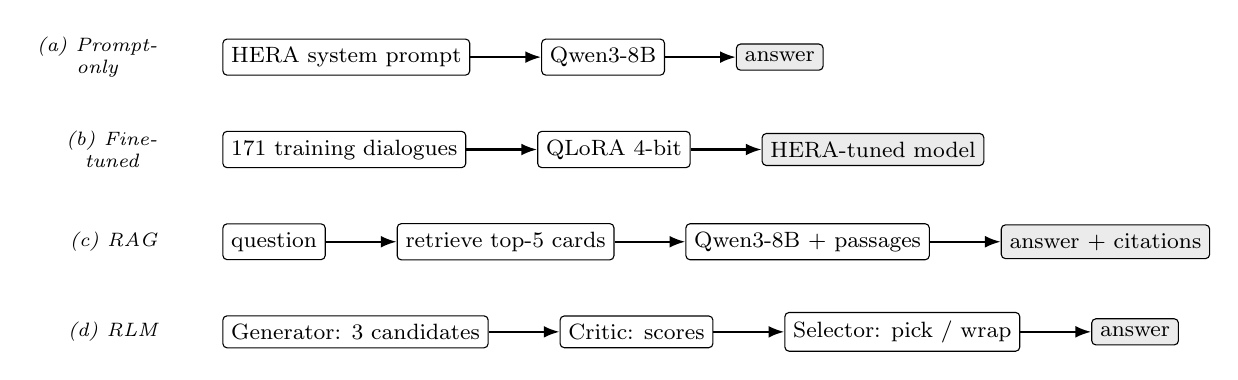
\begin{tikzpicture}[node distance=7mm and 9mm]
  % (a) Prompt-only
  \node[box] (a1) {HERA system prompt};
  \node[box, right=of a1] (a2) {Qwen3-8B};
  \node[boxg, right=of a2] (a3) {answer};
  \node[lab, left=7mm of a1] {(a) Prompt-\\only};
  \draw[arr] (a1) -- (a2); \draw[arr] (a2) -- (a3);
  % (b) Fine-tuned
  \node[box, below=7mm of a1.south west, anchor=north west] (b1) {171 training dialogues};
  \node[box, right=of b1] (b2) {QLoRA 4-bit};
  \node[boxg, right=of b2] (b3) {HERA-tuned model};
  \node[lab, left=7mm of b1] {(b) Fine-\\tuned};
  \draw[arr] (b1) -- (b2); \draw[arr] (b2) -- (b3);
  % (c) RAG
  \node[box, below=7mm of b1.south west, anchor=north west] (c1) {question};
  \node[box, right=of c1] (c2) {retrieve top-5 cards};
  \node[box, right=of c2] (c3) {Qwen3-8B + passages};
  \node[boxg, right=of c3] (c4) {answer + citations};
  \node[lab, left=7mm of c1] {(c) RAG};
  \draw[arr] (c1) -- (c2); \draw[arr] (c2) -- (c3); \draw[arr] (c3) -- (c4);
  % (d) RLM
  \node[box, below=7mm of c1.south west, anchor=north west] (d1) {Generator: 3 candidates};
  \node[box, right=of d1] (d2) {Critic: scores};
  \node[box, right=of d2] (d3) {Selector: pick / wrap};
  \node[boxg, right=of d3] (d4) {answer};
  \node[lab, left=7mm of d1] {(d) RLM};
  \draw[arr] (d1) -- (d2); \draw[arr] (d2) -- (d3); \draw[arr] (d3) -- (d4);
\end{tikzpicture}}
\caption{The four copilot architectures, all built on the same locally-run Qwen3-8B
model. (a) prompt-only uses just the HERA system prompt; (b) the fine-tuned model bakes
the HERA behaviour into the weights via QLoRA; (c) RAG retrieves and cites the relevant
regulatory cards at every turn; (d) the multi-agent RLM proposes, critiques, and selects
a question each turn (a separate synthesiser writes the final report).}
\label{fig:arch}
\end{figure*}
\subsection{Prompt-only (baseline)}
The simplest approach gives the model nothing but the HERA system prompt and lets it
converse. It is the natural baseline: no training, no extra machinery, instant to set up,
and very fast at run time. Its weakness is that it can only draw on what the base model
already happens to know about regulation; its answers can be generic, and it may
confidently cite an article that does not exist. It is, in effect, a knowledgeable
generalist who has skimmed the topic but has no reference book open in front of them.
\subsection{Fine-tuned model (QLoRA)}
The second approach teaches the base model to behave like HERA by training it on
the 171 dialogues. Full fine-tuning of an eight-billion-parameter model is far beyond a
single consumer GPU, so we used QLoRA \citep{dettmers2023qlora}, which combines low-rank
adapters \citep{hu2022lora} with 4-bit quantisation: instead of updating all the weights,
it trains a small number of extra parameters on top of a compressed model. After
training, the adapter is merged back and the model is again quantised to 4~bits so it can
run locally. The appeal is that the HERA style becomes part of the model itself, with no
retrieval needed at run time. The risk is equally clear: with little training data and
heavy compression, quality can degrade, a risk that, as Section~\ref{sec:results}
shows, materialised.
\subsection{Retrieval-augmented generation (RAG)}
The third approach keeps the base model unchanged but gives it an open reference book.
At every turn, the system takes the current conversation, retrieves the five most
relevant regulatory cards from the vector index, pastes them into the prompt, and asks
the model to ground its answer in them and to cite them \citep{lewis2020rag,
gao2023retrieval}. The advantages fit our problem well: answers are anchored in real
regulatory text rather than in the model's memory, hallucinations are reduced, and the
knowledge can be updated simply by editing a card, with no retraining required. The cost is
that quality depends on the retrieval step, and the longer prompts make each turn somewhat
slower.
\subsection{Multi-agent reasoning (RLM)}
The fourth approach turns one turn of conversation into a little team effort, following
the Generator/Critic/Selector design of \citet{deng2025ethical} and the broader idea of
letting a model criticise and refine its own output \citep{shinn2023reflexion,
madaan2023selfrefine}. A Generator proposes three candidate questions, each
targeting a different, preferably uncovered, dimension. A Critic scores the three
on relevance, depth and novelty. A Selector then either asks the strongest
question or decides the conversation has covered enough and wraps up. A fourth role, the
Synthesiser, writes the final risk report. The promise of ``propose several,
critique, then choose the best'' is deeper and more on-target questions for the same base
model. The price is that each turn now costs about three times as many model calls, and
there are more moving parts that can fail.
\section{Evaluation protocol}
\label{sec:eval}
How do you decide which of four conversational systems gives better advice? Our guiding
principle was that every approach must receive exactly the same inputs, so that we
only ever compare how they reason. Figure~\ref{fig:eval} shows the set-up.
\begin{figure}[t]
\centering
\resizebox{0.95\columnwidth}{!}{%
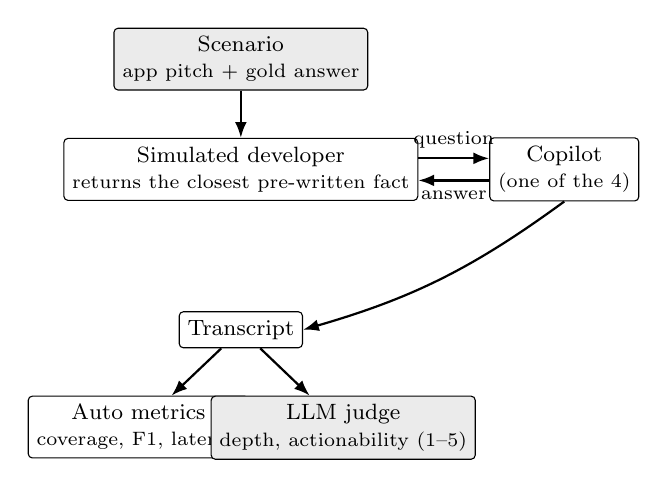
\begin{tikzpicture}[node distance=6mm and 9mm]
  \node[boxg] (sc) {Scenario\\\scriptsize app pitch + gold answer};
  \node[box, below=of sc] (dev) {Simulated developer\\\scriptsize returns the closest pre-written fact};
  \node[box, right=of dev] (cop) {Copilot\\\scriptsize (one of the 4)};
  \node[box, below=14mm of dev] (tr) {Transcript};
  \node[box, below=of tr, xshift=-13mm] (m) {Auto metrics\\\scriptsize coverage, F1, latency};
  \node[boxg, below=of tr, xshift=13mm] (j) {LLM judge\\\scriptsize depth, actionability (1--5)};
  \draw[arr] (sc) -- (dev);
  \draw[arr, transform canvas={yshift=1.4mm}] (dev) -- (cop) node[midway,above,font=\scriptsize]{question};
  \draw[arr, transform canvas={yshift=-1.4mm}] (cop) -- (dev) node[midway,below,font=\scriptsize]{answer};
  \draw[arr] (cop.south) to[bend left=10] (tr.east);
  \draw[arr] (tr) -- (m); \draw[arr] (tr) -- (j);
\end{tikzpicture}}
\caption{Evaluation protocol. Each of the four copilots talks to the same deterministic
simulated developer over a scenario; the resulting transcript is scored both by automatic
metrics and by an LLM judge.}
\label{fig:eval}
\end{figure}
\paragraph{Scenarios.}
We wrote 25 realistic mHealth scenarios, each with a short app description, a
developer persona, and a hand-written ``gold answer'': the dimensions that should be
raised, the risks that should be found (with a severity), the mitigations a good copilot
would suggest, and the regulations that should be cited. The set spans all seven pillars,
includes both AI and non-AI apps, and covers European and Swiss markets, so that no single
approach can win just by specialising in one kind of app.
\paragraph{The simulated developer.}
The key methodological choice is how the ``developer'' answers. If we let a free language
model improvise, each approach would receive different information and the comparison
would be meaningless. Instead, the developer is deterministic: every scenario comes
with a pool of pre-written facts, and when the copilot asks a question we embed it and
return the single most relevant unused fact, measured by cosine similarity against a fixed
threshold. A sharper question lands on a more relevant fact, so the developer's
responsiveness itself becomes a quiet signal of question quality. If nothing relevant
matches for several turns in a row, the conversation stops before it starts to loop.
\paragraph{Automatic metrics.}
From each transcript we compute four mechanical measures. Coverage is the share of
the gold dimensions that the copilot actually raised (recall). Relevance is the
share of the questions asked that touch a relevant dimension (precision). Risk
accuracy is an F1 score on the named risks against the gold answer. Latency is the
average time per turn. These are strict, regex-based counts: they are objective but
unforgiving, and they penalise a useful answer the moment it mentions a dimension that the
narrow gold list did not anticipate.
\paragraph{LLM judge.}
Because strict counting misses the real quality of advice, a separate language model acts
as a judge \citep{zheng2023judging}. It reads each transcript, together with the gold
dimensions, and rates it on two 1-to-5 scales: Depth (does the copilot drill
into the specifics of this app and the precise article that applies, or stay
generic?) and Actionability (could a competent developer implement the suggestions
tomorrow, or are they vague platitudes?). The judge is explicitly told to be strict and
not to inflate scores. The same simulated developer drives every approach, conversations
run for up to ten to twelve turns, and the judge uses a low temperature for stability.
\section{Results}
\label{sec:results}
Table~\ref{tab:results} reports the four approaches on the twenty-five scenarios, on both
the automatic metrics and the LLM judge.
\begin{table*}[t]
  \centering
  \footnotesize
  \setlength{\tabcolsep}{6pt}
  \begin{tabular}{|l|c|c|c|c|c|c|}
    \hline
    \textbf{Approach} & \textbf{Coverage} & \textbf{Relevance} & \textbf{Risk F1} &
    \textbf{Latency (s/turn)} & \textbf{Depth (1--5)} & \textbf{Actionability (1--5)} \\
    \hline
    Prompt-only & 0.322 & \textbf{0.116} & \textbf{0.180} & \textbf{4.26} & 2.48 & 2.20 \\
    \hline
    Fine-tuned (QLoRA) & 0.095 & 0.090 & 0.043 & 15.47 & 1.16 & 1.04 \\
    \hline
    \textbf{RAG} & \textbf{0.359} & 0.092 & 0.152 & 10.85 & \textbf{3.04} & \textbf{2.72} \\
    \hline
    RLM (multi-agent) & 0.261 & 0.062 & 0.087 & 20.72 & 2.40 & 2.08 \\
    \hline
  \end{tabular}
  \caption{Evaluation results over 25 scenarios. \emph{Coverage}, \emph{Relevance} and
  \emph{Risk F1} are automatic; \emph{Depth} and \emph{Actionability} are the LLM judge's
  averages. Best value in each column in bold (lower is better for latency).}
  \label{tab:results}
\end{table*}
The clearest message is that RAG wins on the measures that matter most for
usefulness. It achieves the best dimension coverage (0.36) and, more importantly, the
best scores from the judge on both depth (3.0) and actionability (2.7): grounding each
answer in the retrieved regulatory cards lets it refer to the right article and give
concrete, implementable advice.
The prompt-only baseline is surprisingly strong and by far the fastest
(4.3~seconds per turn, roughly two to five times quicker than the others). It even tops
the strict automatic precision and F1, and lands second behind RAG on the judge. For a
zero-setup approach this is a notable result, and it makes prompt-only a sensible fast
fallback.
The multi-agent RLM does not pay off here. Its scores sit in the middle of the
pack while its latency is the highest of all (20.7~seconds per turn, about three times the
baseline), because every turn runs the model several times. The extra ``propose, critique,
select'' machinery did not translate into better questions for this taxonomy and this base
model.
The fine-tuned model collapsed. It is the weakest approach on every single
measure, with judge scores close to the floor (depth 1.16, actionability 1.04). In its
transcripts it repeats the same templated question turn after turn, invents references,
and sometimes even renames the app. The training itself looked healthy (the validation
loss fell steadily from~2.23 to~1.97 over three epochs with no sign of over-fitting), so
the failure appears at inference time, not during learning. We return to this in the
discussion.
It is worth noting that the automatic precision is low for all four approaches.
This is largely an artefact of the evaluation: the gold list of dimensions is deliberately
narrow, so any extra (and possibly still reasonable) dimension a copilot raises is counted
as a mistake. This is precisely why we do not rely on the mechanical metrics alone, and
why the LLM judge, which reflects the real quality of the advice, carries most of the
weight in our reading of the results.
\section{Discussion and conclusions}
\label{sec:discussion}
\paragraph{What we kept.}
Taken together, the results point to a clear choice. We kept the RAG copilot as
the main system because it gives the best-quality, best-grounded advice and because its
knowledge can be updated simply by editing a regulatory card, with the prompt-only
model retained as a fast fallback. The multi-agent setup was dropped: it was markedly
slower for no measurable gain. The end product is a small, fully local and private
prototype (the model runs on the developer's own machine through Ollama and no data is
sent to any external service), wrapped in a three-page web app (app profile, an
interactive regulation diagram, and the HERA chatbot).
\paragraph{Why the fine-tuned model failed, and why it should not be dismissed.}
The collapse of the fine-tuned model deserves a careful reading, because it is a
limitation of our conditions, not a verdict on the method. Two constraints stacked
up. First, the training set was small: 171 dialogues is enough to nudge a model's style
but thin for reshaping an eight-billion-parameter model. Second, and more decisively, we
were limited by hardware. A full fine-tune of an 8B model needs far more GPU memory than
we had available, so we could only afford QLoRA, a 4-bit adapter on top of an already
compressed model, and we then quantised the merged model to 4~bits again so it would
run locally. This double compression is the most likely cause of the mode collapse we
observed (repeated questions, invented citations, empty reasoning tags). With a
full-precision fine-tune on adequate hardware, more training data, and inference at higher
precision, there is every reason to expect the fine-tuned model to become competitive with,
and possibly stronger than, the prompt-only baseline. In other words, fine-tuning
was not given a fair chance here; the result reflects our budget, not the ceiling of the
approach.
\paragraph{Limitations.}
Beyond the hardware budget, three limitations temper our conclusions. The gold standard is
narrow, which depresses the automatic precision and means those numbers should be read as
trends rather than exact values. The LLM judge, while strict, is a single model, so its
scores carry some variance. And the evaluation covers twenty-five scenarios: enough to see
clear patterns, but not to split hairs over second-decimal differences. Finally, the
current vector index covers the curated regulatory cards rather than the full source
documents, which keeps retrieval focused but bounds how deep an answer can go.
\paragraph{Conclusion and future work.}
We set out to make the maze of digital-health regulation navigable for the people who
build health apps. HERA unifies eight frameworks into an actionable taxonomy of seven
pillars and thirty-eight dimensions, and a retrieval-grounded copilot built on a small,
local model turns that taxonomy into useful, well-sourced advice given early, at design
time. A rigorous comparison of four architectures over twenty-five scenarios shows that
retrieval is the most useful approach today, that a plain prompt is a strong and fast
fallback, and that fine-tuning was held back by hardware rather than by principle. The most
promising next step is therefore to revisit fine-tuning with more data and a full-precision
training run on better hardware, and to combine it with retrieval. Further work includes
broadening the scenario set, using several judges to reduce variance, indexing the full
regulatory documents, and running user studies with real developers to test whether a
copilot like HERA genuinely changes how early risks are caught.
% Custom bibliography entries only
\bibliography{custom}
\end{document}
